% -*- mode: fundamental -*-

% ****************************************************************

\chapter{Introduction}

\markboth{Ch \arabic{chapter}: Introduction}{\copyrightnotice}


\setcounter{page}{1}
% \renewcommand{\thepage}{\arabic{page}}
\renewcommand{\thepage}{\arabic{chapter}-\arabic{page}}

\label{ch_intro}

% ****************************************************************

``Digital Design'' and ``CPU Design'' (or ``Computer Architecture'')
are traditionally taught separately, usually in that order, with
separate textbooks.  Digital Design is usually taught using one of the
traditional hardware design languages Verilog, SystemVerilog or VHDL,
and often makes use of small, often artificial examples.  CPU Design
is often taught without actually designing hardware, relying instead
on textbooks, abstract schematics, and simulators implemented in
software.

This book takes a different approach: we learn about simple CPU
architectures by designing them with a modern Hardware Design Language
(HDL) called BSV, learning Digital Design as an ongoing, intertwined
accompanying topic.  Each Digital Design example will be taken
directly from the CPU Design, so that the example's use-case (context)
is always perfectly clear, and the reader always has a clear sense of
the purpose of the example.

The CPUs we design here will execute instructions from the RISC-V
Instruction Set Architecture (ISA), which is an industrial-strength
ISA (with many commerical implementations).  Our designs will be
simple (typical of small, embedded systems and micro-controllers, not
laptops/workstations or servers).

Figure~\ref{Fig_Topics} shows the broad range of topics in which a CPU
designer needs to engage.
\begin{figure}[htbp]
  \centerline{\includegraphics[width=6in,angle=0]{Figures/Fig_Topics}}
  \caption{\label{Fig_Topics}Topics covered in this book (in red text in red box)}
\end{figure}
Some of the early topics are not RISC-V implementation-specific:

\begin{itemize}

\item The first step is to understand the RISC-V ISA itself.  What are
    RISC-V instructions, how are they coded in bits, and what do they
    mean?  This topic is not a focus of this book (for which there are
    plenty of textbooks and other educational materials available),
    but understanding the ISA is of course a prerequisite to informing
    our design, so we provide a brief overview in
    Chapter~\ref{ch_ISA}.

    The RISC-V ISA has many options; our focus in this book will be on
    a small ``standard'' subset that is adequate for small embedded
    systems:

    \begin{tightlist}
		  
      \item The so-called ``RV32I'' subset from the RISC-V
            Unprivileged ISA spec: basic integer arithmetic and logic
            operations; branch and jump; load and store.

      \item A few elements from the RISC-V Privileged ISA spec for
            handling exceptions: Control and Status Registers (CSRs),
            traps and trap-handling.

    \end{tightlist}

\item In order to run actual RISC-V programs on our implementations,
      we need to undertand how to use the \emph{riscv-gcc} compiler to
      compile C and RISC-V Assembly Language programs into RISC-V
      binaries (so-called ``ELF'' files).  Another useful tool is
      \emph{riscv-objdump}, which can disassemble the binary back into
      assembly-language text. This is useful for debugging our
      implementation, so that we can understand execution
      instruction-by-instruction, and diagnose anything that goes
      wrong.

      How to install and use these tools is not a focus of this book
      but of course we need to use these tools to produce programs to
      run on our implementations.

\end{itemize}

So, far, all this is not implementation-specific, {\ie} it is generic
information about RISC-V.  The following topics dive into
implementations.


\begin{itemize}

\item A RISC-V CPU and system can be \emph{modeled} in a simulator
      coded in C (say).  Such a C-based simulator is compiled (with
      \emph{gcc}, say) and run like any other C program. We will not
      be discussing this much in this book.

\item We will code our hardware design in the BSV HL-HDL.  We will use
      BSV not just for the CPU itself, but also for the ``system''
      components around it: an interconnect, Memory, UART and GPIO.

\item We will use the \emph{bsc} compiler to translate our BSV code
      into Verilog RTL.

\item We will learn how our Verilog RTL can directly be simulated in a
      Verilog simulator.  We will use the free, open-source
      ``Verilator'' simulator, but you can also run it on any other
      Verilog simulator, available from a number of providers.

      This will provide an exact, cycle-by-cycle accurate simulation
      of the very same design that we'll run later on an FPGA.  This
      is invaluable for debugging the hardware design, because the
      turnaround time to fix a problem and run a new simulation is
      very short (minutes) compared to creating a new version for an
      FPGA (several hours).

      Of course, Verilog simulation will run much more slowly (10,000x
      or more slower) compared to an FPGA, and so is useful primarily
      for early debugging and analysis of the design, running on small
      RISC-V programs.

\item When we execute our Verilog RTL hardware design in Verilog
      simulation (where the hardware design itself is executing a
      RISC-V binary program), it will produce a trace file describing
      events during the simulation.  We will learn how to analyze
      these traces to identify bugs and bottlenecks in our design,
      from which we can correct design errors and possibly improve
      performance.

\item We will discuss how to process our Verilog RTL through an FPGA
      synthesis tool to create an FPGA bitfile which can then be
      loaded into an FPGA and executed.

      Although it can be synthesized and run on a number of FPGAs from
      different vendors, in this book we'll discuss how to build and
      run it for an FPGA on the Amazon AWS cloud.

\item Our Verilog RTL can also be processed through ASIC synthesis
      tools targeting ASIC fabrication.  We will not be dicsussing
      this much in this book.

\end{itemize}

% ================================================================

\section{Drum and Fife, the two RISC-V implementations designed in this book}

We will create two hardware RISC-V designs, called Drum and Fife,
illustrated in Figure~\ref{Fig_Two_Microarchitectures}:
\begin{figure}[htbp]
  \centerline{\includegraphics[width=6in,angle=0]{Figures/Fig_Two_Microarchitectures}}
  \caption{\label{Fig_Two_Microarchitectures}Two CPU implementations (microarchitectures)}
\end{figure}

\begin{itemize}

  \item Drum is a \emph{non-pipelined} implementation which will
        familiarize us with all the basic concepts and flows (the
        RISC-V ISA, preparing and running a RISC-V binary to run on
        the design, analysing traces), without being distracted by the
        complexities of pipelining for high performance.

  \item Fife is a 5-6 stage pipelined design, which is a
        microarchitectural change focused on higher performance
        (speed) than Drum. The design includes simple
        branch-prediction, register read/write hazard management,
        in-order retirement of instructions, and speculative stores to
        memory using a store-buffer.

\end{itemize}

The two designs will share a large part of the BSV code that
implements the essential semantic functionality of the RISC-V ISA.  By
discussing this shared code in the simpler Drum, the Fife chapters can
focus purely on the new issues raised by pipelining (and which are, in
fact, not RISC-V specific, but common to all pipelined CPU designs).

Drum and Fife execute exactly the same binaries; the only difference
will be in Fife's superior performance (speed).

As we work through the two designs, we will concurrently learn how to
code in BSV, the HL-HDL for our designs.  BSV is a modern, high-level
HDL taking inspiration from modern software programming languages, in
particular the Haskell functional programming language and a class of
formal specification languages for concurrent programming (including
Term Rewriting Systems, Unity, TLA+, and Event-B).  BSV is not just
for CPU design; like Verilog and SystemVerilog, it is a ``universal''
language for any digital design, whether related to CPUs or not.
Appendix~\ref{apx_Why_BSV} has a more detailed justification of our
choice of BSV over other hardware design languages like Verilog,
SystemVerilog, VHDL or Chisel.

% ================================================================

\subsection{Drum and Fife source codes}

The full source codes (BSV) for Drum and Fife are included with this
book.  Excerpts of that code are taken, as-is, for inclusion in this
book.  Excerpts look like this:

\input{Code_Extracts/CPU_IFC.tex}

The label on the top border of the box indicates file
(\verb|src_Common/CPU_IFC.bsv|) from which this has been extracted,
and the starting line number (27) in the file.  The ``\verb|...|''
indicates we have \emph{elided} some lines from the source file which
are not directly relevant to the current discussion.

We recommend, as you read the book, that you also keep open a
text-editor, in which you can simultaneously view the actual sources.

% ================================================================

\section{General structure and operation of digital circuits}

In this section we provide some general intuitions of how digital
circuits operate, sufficient to allow us to proceed with design.

Digital hardware is driven by a clock, an electrical signal that
oscillates between a low voltage and a high voltage, with sharp
transitions between the two, at regular intervals (it is therefore
sometimes called a ``square'' wave).  This is illustrated in
Figure~\ref{Fig_Clock_1}.

\begin{figure}[htbp]
  \centerline{\includegraphics[width=6in,angle=0]{Figures/Fig_Clock}}
  \caption{\label{Fig_Clock_1}A clock signal}
\end{figure}

Nowadays, clock cycle times/periods are typically measured in
nanoseconds. For example, a 100 MHz clock has a 10ns cycle time.

Any value that must be visible from one clock to the next must be
stored in a \emph{state element} (a component that can ``remember''
values, {\ie} has \emph{state}, like a register, FIFOF, buffer,
memory, ...).

Digital circuits are composed of state elements and
\emph{combinational circuits} connecting outputs of state elements to
inputs of state elements, as illustrated in
Figure~\ref{Fig_BSV_Digital_Circuits}.  State elements are
\emph{storage} elements.  Combinational circuits are \emph{acyclic}
networks of \emph{logic gates}.  A logic gate is a circuit that
``instantaneously'' computes a boolean function (such as AND, OR, NOT,
XOR, ...) of its boolean inputs.

\begin{figure}[htbp]
  \centerline{\includegraphics[width=6in,angle=0]{Figures/Fig_BSV_Digital_Circuits}}
  \caption{\label{Fig_BSV_Digital_Circuits}
           Digital circuits consist of state elements interconnected
	   with acyclic combinational circuits}
\end{figure}

Any digital circuit repeatedly performs the following:

\begin{itemize}

\item After each ``posedge'' (positive edge of a clock), the
      combinational circuits compute new inputs for all state
      elements, based on the current values in state elements

\item At the next posedge, these new input values are stored into the
      state elements.

\end{itemize}

The above description is a simplification, or an idealization.
Physics and circuit silicon technology dictates how long an electrical
signal takes to propagate from the output of a state element and
through a combinational circuit before it arrives at the input of a
state element.  For correct operation, the clock period needs to be
greater than this, to allow signals that are inputs to state elements
to ``settle down'' and be steady when they are captured on the next
clock edge.

\index[BSV]{Digital Abstraction, The}

In the \emph{Digital Abstraction} we assume this condition is met, and
we idealize wire and combinational circuit delays as taking zero time.

% ----------------

\vspace{1ex}

NOTE: \fbox{\small
\begin{minipage}{5in}

\begin{itemize}

 \item Advanced digital ciruits may have multiple clocks driving
       different parts of the circuit.

 \item Advanced digital ciruits may vary the clock speed dynamically,
       to match power consumption to current performance demands
       (higher speeds $\Rightarrow$ more power consumption).

 \item Some digital ciruits use the negative edge (``negedge'') of the
       clock insted of the posedge.

 \item Advanced digital ciruits may use both the posedge and the
       negedge of the clock.

\end{itemize}

\end{minipage}}

\vspace{1ex}

% ----------------

% ----------------------------------------------------------------

\subsection{Computer memories; split-phase and pipelined acces}

A computer memory is a packaged device:
\begin{itemize}

 \item To read memory, we present a \emph{read request} at its inputs,
       with an \emph{address}; \\
       the memory provides a \emph{read response} at its outputs,
       containing the addressed data.

 \item To write memory, we present a \emph{write request} at its
       inputs, with an address and data; \\
       the memory provides a \emph{write response} at its outputs,
       containing an ``ok'' status.

\end{itemize}

\index[BSV]{RAM (Random Access Memory)}
\index[BSV]{Memory!RAM (Random Access Memory)}

Because we access memory by presenting an address identifying a
location in memory, they are called RAMs (Random Access Memories).
Memories are, nowadays, typically byte-addressed, {\ie} each address
identifies a particular byte in memory.  Memory access instructions in
the CPU can typically specify a \emph{size} in bytes, typically 1, 2,
4 or 8 bytes.

\index[BSV]{SRAM (Static RAM)}
\index[BSV]{DRAM (Dynamic RAM)}

\index[BSV]{Memory!SRAM (Static RAM)}
\index[BSV]{Memory!DRAM (Dynamic RAM)}

\index[BSV]{Memory Hierarchy}

All computers contain RAMs of various kinds.  Two major categories are
SRAMs (Static Random Access Memories) and DRAMs (Dynamic Random Access
Memories).  For the same size, SRAMs are more expensive (more silicon
area, more power consumption) and faster (less time to access a
location) compared to DRAMs.  Thus, computers typically use SRAMs for
smaller memories ``closer'' to the CPU (such as caches) and DRAMs for
``main memory'' which is ``more distant'' from the CPU.  These
arrangements are also referred to as a ``memory hierarchy''.  Cache
sizes typically range from the 10s of kilobytes to 100 megabytes,
whereas main memories can range into several gigabytes.

\index[BSV]{Split-phase memory access}
\index[BSV]{Memory!split-phase access}

Typically, (for any memory larger than a few kilobytes), the response
is available \emph{one or more clocks after} the inputs were
presented.  We also say that memory accesses are
\emph{split-phase}---requiring temporally separated request-production
and response-consumption.  This is illustrated in
Figure~\ref{Fig_BSV_Split_Phase_Mem}.
\begin{figure}[htbp]
  \centerline{\includegraphics[width=6in,angle=0]{Figures/Fig_BSV_Split_Phase_Mem}}
  \caption{\label{Fig_BSV_Split_Phase_Mem} Split-phase memory access}
\end{figure}

Memory systems are also often pipelined: the CPU can issue a
continuous stream of requests, and the the memory sends back a
continuous stream of responses.  The CPU does not have to wait for the
first response before issuing its second request.  Thus, in
Figure~\ref{Fig_BSV_Split_Phase_Mem}, we have labeled the arrows to
and from memory with little red symbols representing \emph{queues} or
FIFOs (First-In-First-Out).  The whole path from the CPU to memory and
back can be regarded as a queue, with requests entering and responses
exiting the queue.

\index[BSV]{Memory!latency}

The delay from when the CPU issues a request until it receives the
corresponding response is called \emph{memory latency}.  This is
typically measured in clock cycles or in real-time units (nanoseconds,
microseconds).

\index[BSV]{Memory!bandwidth}

The rate at which requests and responses are pumped through the memory
system is called \emph{memory bandwidth}.  This is usually measured in
transactions-per-second, or requests-per-second, or in
bytes-per-second where the bytes usually refer to data bytes
transferred, excluding address bytes and other overhead bytes.

Both latency or bandwidth can vary, based on the byte-size of the
access, whether or not requests encounter cache-misses, virtual-memory
page faults, cache-coherence delays, and so on.

% ================================================================

\section{Additional Resources for this Textbook/Course}

Chapter~\ref{ch_BSV_further_study} has suggestions for further study
of BSV.

Chapter~\ref{ch_RISCV_further_study} has suggestions for further study
of RISC-V and CPU design.

Appendix~\ref{apx_resources} has a detailed listing of resources
(documents and software tools) needed for this book, and for further
reading.

This book also contains a Glossary of terms and abbreviations, and a
detailed index.

% ****************************************************************
